\documentclass[apj]{emulateapj}

\usepackage{graphicx}
\usepackage{amssymb}
\usepackage{amsmath}
\usepackage{natbib}
\bibliographystyle{apj}
\usepackage[breaklinks,colorlinks,citecolor=blue,linkcolor=magenta]{hyperref}
\shorttitle{Short Title}
\shortauthors{Zhou et al.}

%%% new command %%%
\newcommand{\ima}{\texttt{ima} files }
\newcommand{\flt}{\texttt{flt} files }
\newcommand{\eps}{$\mathrm{e}^{-}/\mathrm{s}$}
\begin{document}
\title{Variability of Planetary Mass Companion 2M1207 B}
\shorttitle{Variability of 2M1207 B}
\author{Yifan Zhou, Daniel Apai, Glenn Schneider, ...}
\affil{The University of Arizona}

\begin{abstract}
...
\end{abstract}

\keywords{kw1, kw2, ...}
\maketitle
%
\section{Introcduction}

\section{Observation}
We took high contrast direct imaging observation of 2M1207 system on
UT 2014 April 11 using HST.  (\textit{HST} Proposal GO-13418, PI:
D. Apai). The data were acquired with the Wide Field Camera 3 (WFC3)
in filter F125W ($\lambda_{\mbox{pivot}}$ = 1245.9 nm, full width at
half maximum (FWHM) = 301.5
nm) and F160W ($\lambda_{\mbox{pivot}}$ 1540.52, FWHM = 287.9 nm)
using the $256\times256$ sub-array mode. We observed 2M1207 system in
six contiguous HST orbits and obtained a data-set that have a temporal
resolution of $\sim1.5$ minutes and baseline of 8 hours and 40
minutes, interrupted by Earth occultaions of 58 minutes every  94 minutes.


The observations was initially designed to apply two-roll
point spread function (PSF) subtraction (e.g. \cite{Song2006}) to remove the background light
from the primary star. The telescope roll angles for data taken in
orbit 1, 3, 5 and those taken in orbit 2, 4, 6 differed by
$25^{\circ}$, thus the roll displacement of the companion is $0.34''$
that is 2.75 and 2.30 resolution elements in F125W and F160W respectively.
In each orbit we took a sequence of 13 SPARS10 exposures with
NSAMP=10, alternating between F160W and F125W filters, with 2-3
identical exposures in one exposure sequence. To improve PSF sampling
and reduce the risk caused by bad pixels, we applied standard 4 point
dithering. In each orbit, exposures were taken with dithering position
1 -- 4 sequently. Over the 6 orbits, we obtained 70 multi-acuum images for filter
F125W and 64 images for filter F160W with exposure time of 88.4
seconds for both two filters.


\section{Data Reduction}

Through the whole analysis, we used the \flt that were produced by
WFC3's \texttt{calwfc3} pipeline. The \flt were reduced with
calibration steps including dark current correction, non-linearity
correction, and flat field correction. A further step of up-the-ramp
fit was applied to combine all non-destructive reads and remove cosmic
rays. Although \cite{Mandell2013} stated that WFC3 IR time series
extract from {\flt} have a rms 1.3 times larger than that obtained
from {\ima}, \flt keeps all pixels of the image of 2M1207 A
unsaturated, while in 80\% of non-destructive reads the cores of
2M1207 A are saturated. Thus \flt help better align the images for
primary subtraction, and separate the flux of 2M1207 B from that of
2M1207A.

The small angular separation of 2M1207 A and B (as shown in Figure
\ref{fig:1}) makes precise primary star subtraction and photometry
very difficult. On the under-sampled WFC3 IR detector (plate scale
$\sim 0.13''\mbox{pixel}^{-1}$ \cite{dressel2012wide}), the primary
and the secondary only separate by $\sim 6$ pixels, which is about 5
times of the FWHM of the PSF. In addition, under-sampling causes
significant artifacts when shifting the images for registration no
matter what interpolation method is used.

\begin{figure*}
  \centering
  \plottwo{original}{subtracted}
  \caption{WFC3 F160W images of 2M1207A system. Upper: original image,
    lower: residual model and primary PSF subtracted. The image of
    2M1207 B is overshadowed by the halo of the image of 2M1207A and
    can be hardly seen from the original image. With a hybrid PSF
    (residual + Tiny Tim PSF) subtraction, the image of 2M1207 B is
    clearly displayed.}
  \label{fig:1}
\end{figure*}

\subsection{Tiny Tim PSF Photometry}
To over come the difficulty, we make use of the Tiny Tim PSF simulator
to pursue high precision photometry under this extreme
circumstance. Tiny Tim can produce model PSF based on the filter,
spectrum of target, focus status, and the telescope jitter. One
significant advantage of Tiny Tim PSF over empirical PSF is that Tiny Tim can
produce Nyquist sampled PSF, which makes image shifting and interpolation
rather straight forward. One essential disadvantage of Tiny Tim is
that the model PSFs have significant systematic
errors. \cite{Biretta2014} demonstrated that the diffraction
spikes and coma are not well simulated with Tiny Tim for WFC3 IR
images. However, using the 6-orbit long time series, we are able
to well characterize the difference of model PSFs and empirical PSFs.
By modeling the difference and combining it with model PSFs, we can
produce high quality hybrid PSFs to significantly improve the PSF
simulation and PSF photometry.

We started the reduction by making bad pixel masks for every
image. Pixels with data quality flags ``bad detector pixels'' (DQ = 4),
``unstable response'' (DQ = 32), and ``bad or uncertain flat value'' (DQ =
512) were masked out and excluded from further analysis as suggested
by previous transit exoplanet
spectroscopic observations\citep[e.g.][]{Berta2012, Kreidberg2014}.

We then produced a list of 10x over-sampled PSFs based on the
positions and spectrum \citep{Bonnefoy2014} of 2M1207 A with different
telescope jitter ranging from 0 to 50 $\mbox{mini-arcsec s}^{-1}$ in
both $x$ and $y$ directions. We used the new set of Tiny Tim
parameters provided by \cite{Biretta2014} to better model the cold
mask, diffraction spikes, and the coma. The focus parameters were
calculated using the model listed on the STScI
website\footnote{\url{http://www.stsci.edu/hst/observatory/focus/FocusModel}}. The
PSFs were registered with the original image by searching on a dynamic
grid and minimizing the difference of observation and model PSF at a
region centered on 2M1207 A with the image of 2M1207 B mostly
excluded. The best fitted primary star position and telescope jitter
were obtained in this step. Then, we generated the PSF for 2M1207 B
based on its position on detector, spectrum \citep{Patience2010}, and
the telescope jitter that had been obtained above. In the final step,
we combined the two PSFs together. We fixed the position of the
primary as it had been fitted in the first step and fitted for the
amplitudes of the two PSFs and the precise position of the
secondary. Since the total fluxes of the model PSFs were normalized to
unity as default, the fluxes of 2M1207 A and B were solely represented
by the amplitude of the two PSFs coordinately.

Because of the systematic errors of the Tiny Tim PSF, the quality of the
fitting is not optimistic. The reduced $\chi^{2}$ values were at level
of $\sim10$. However, we found that the residual patterns were very
stable among the image that have the same dithering position and
telescope rolling. Therefore, we median combined the residual images
that have the same dithering position and telescope rolling angle to
construct 8 residual models (4 dithering position $\times$ 2 telescope
rolling angle) for each filter. We pre-subtract the corresponding
residual from the original image and repeated the procedure that
listed above. Using this extra-step, the reduced $\chi^{2}$
greatly decreased to around unity.


\subsection{Uncertainty analysis}

\subsubsection{White noise}
The scatters of the photometric measurements are dominated by photon
noise. Uncertainties of one photometric measurement was combined by
photon noise of every pixel during the PSF fit. The photon noises for
2M1207B photometry in F125W and F160W are 1.33\% and 1.02\%,
respectively, and are at the same level of the scatter of the
photometric time series.

\subsubsection{Flat field uncertainties}
In our observation, 2M1207 B were taken exposure at 8 different spots
on the detector (2 rolls $\times$ 4 dithering
positions). The uncertainties in the flat field are potential sources of variation. The uncertainty of WFC3 IR pipeline flat field
is $\sim 1\%$ \citep{dressel2012wide} and our time resolved observation for another target
demonstrate that aperture photometry for exposures taken at different
dithering position have scatterings at the same level.

Flat field uncertainties have smaller effects on PSF photometry than
aperture photometry since multiple pixels are fitted
simultaneously. To verify this, we multiplied an artificial flat field
error mask that is a uniform distributed Gaussian noise array with
mean of 1 and sigma of 1\% to every image, and repeat the PSF
photometry routine with the error-applied images. We obtained almost
same photometry measurements as the original.

However, PSF profile changes with different exposure positions due to
pixelation, especially for the case that WFC3 IR is significantly
under-sampled. Also, the flat fields may potentially have large scale
structures \citep{dressel2012wide}. Because of these factors, The
fluxes for both 2M1207 A and B are clearly correlated with the
dithering position. To reduce the correlation, we normalize each group of exposures
that have the same dithering position and roll angle individually --
we took the median of the fluxes that were measured from these
exposures as normalization factors and devided them from every photometric
measurement. Because the normalization factor for each group of
exposures is calculated across the whole observation, this
normalization step have negligible impacts on variability analysis.

\subsubsection{Validity tests for the variability}

\begin{figure*}
  \centering
  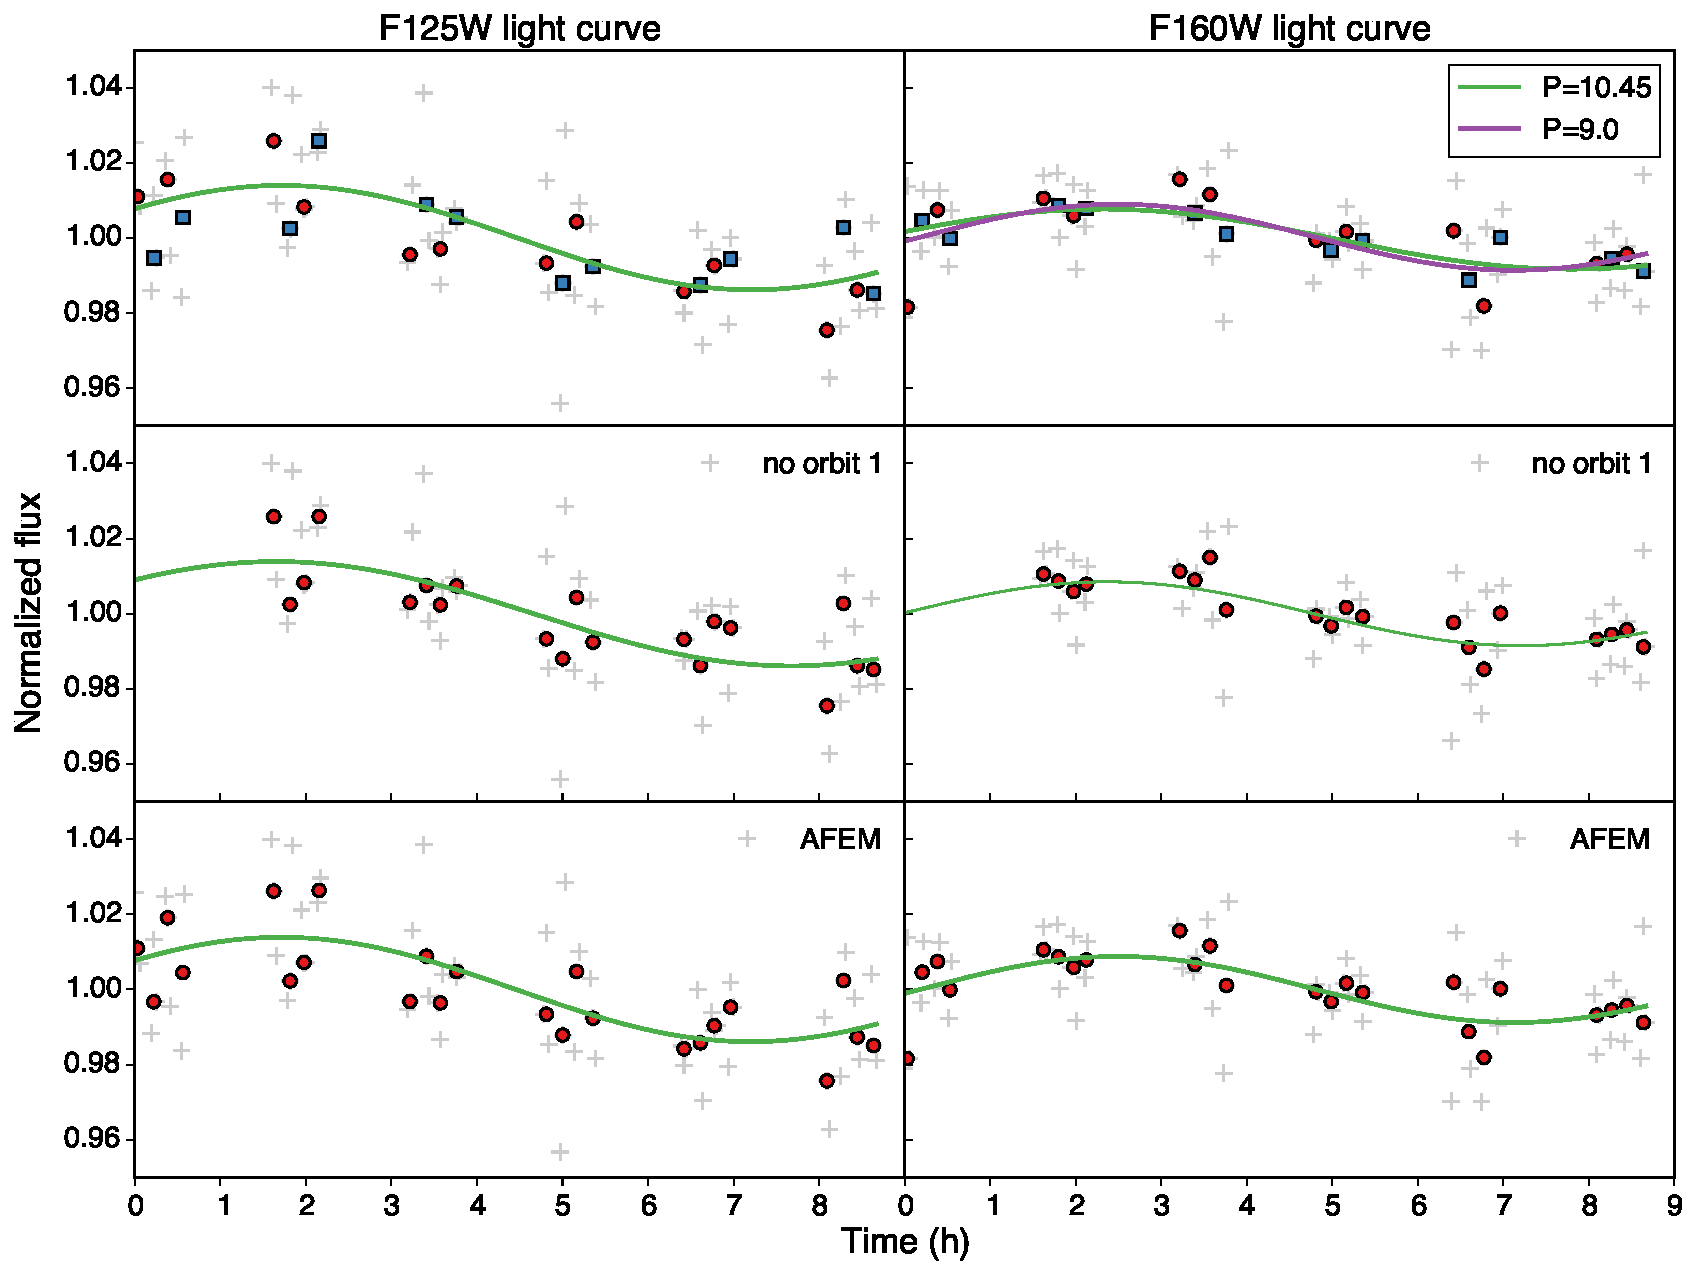
\includegraphics[width=\textwidth]{systematics}
  \caption{Normalized light curves for 2M1207B with filter F125W
    (left) and F160W (right). Original photometric measurements are
    plotted with gray crosses. The two halves of data are binned
    individually, and plotted with red points (first half) and blue
    squares (second half). The F160W light curves are plotted with two
  fitted sinusoidal curves, The green curve is fitted with
  the period fixed to be same as the F125W and the purple curve is
  fitted with all parameter set free.}
  \label{fig:2}
\end{figure*}

Because the aim of this letter is to search for temporal change, it is
essential to exclude the possibility that variability is systematic
artifacts.

 We fitted sinusoidal waves to both of the F125W and F160W light
 curves to preliminarily quantify the variability. The periods of the
 best fitted sine function of the two light curves are similar, 10.9
 hour for F125W and 9.3 hour for F160W, and the periods fitted here
 are not related with any WFC3 instrumental periods. The similarity of
 the period measurements is a proof that the variability is physical.

 Due to image persistence effect, the first orbit of HST observation
 is often problematic, and is neglected by several analyses
 (\textbf{citation?}). In our analysis, the fluxes measured from 2M1207 A are
 significantly lower in the first lower (Figure \ref{fig:3}) than
 those measured from rest fo the orbits. The exposure levels at the
 pixels of the peak of the PSF of 2M1207 B are less than 10000 e$^{-}$
 for both two colors, thus image persistence is less of an issue for
 2M1207 B. To further exclude this effect, we fitted sinusoidl waves
 to the light curves without using the first orbit, and obtained
 similar results.

 To rule out the possibility that the variability is introduced by
 data reduction, e.g., the normalization step, we split the data into
 two halves -- the first half is the data taken at dithering position 1
 and 3, and the second half is that for ditheirng position 2 and
 4. For each half, we repeat the analysis independently. For both of
 F125W and F160W, two halves demonstrated similar trend of
 variability as shown in Figure \ref{fig:2}.
 % \begin{itemize}
% \item the source of the scattering -- 
% \item flat field uncertainty -- adding artificial flat field error mask
% \item validity of the variability\\
%   -- both filter demonstrate similar period of variability\\
%   -- split the data into two half, the trend in two halves of data
%   looks similar.
%   -- fix the position does not change the light curve
% \item uncertainty of sinusoidal curve fit
%   -- carry out a mcmc fit? is it worth doing this.
% \end{itemize}

\section{Result}

\begin{figure*}
  \centering
  \plotone{sineCurveFit_binCombined}
  \caption{Normalized light curves for 2M1207 B (upper) and A (lower)
    with filter F125W (left) and F160W (right). Individual photometric
  measurement are plotted in gray crosses and binned photometry are
  plotted with red points. Best fitted sinusoidal waves are plotted
  with blue solid lines.}
  \label{fig:3}
\end{figure*}

We obtained high signal to noise photometry series for both 2M1207 A
and B (Figure \ref{fig:3}). On average, the photometric contrast is $6.52\pm0.03$ for
F125W and $5.77\pm0.02$ for F160W. The difference of F125W contrast
from that measured in J-band \citep{Mohanty2007} and
F160W contrast from that measured with NICMOS F160W 
\citep{Song2006} is due to the different throughput profiles of the
filters.

Although the photometric time series demonstrate relatively large
scattering, both F125W and F160W light curves demonstrate sinusoidal
shape with clear temporal variability. We fitted sine waves to the two
light curves using least square optimization, and determined the
periods and variation amplitudes. The best fitted periods for F125W
and F160W are 10.9 and 9.3 hour correspondingly. The amplitudes for
the normalized light curves are 1.4\% and 0.9\% for F125W and F160W
light curves.


\begin{figure*}
  \centering
  \plottwo{periodDistr}{amplitudeDistr}
  \caption{Distributions for periods (left) and amplitudes(right) for the light
    curve of F125W and F160W. The bin size for histograms of period is
  0.25 hour and for that of amplitude is 0.5\%. Histograms are
  normalized in the way that total area of the histogram equals to
  1. In the right panel, Gaussian profiles are fitted to the
  histograms and plotted in solid lines.}
  \label{fig:4}
\end{figure*}

To constrain the uncertainties of the least square optimization
results, we used a Monte Carlo(MC) method to improve the fitting. We
generated a series of random Gaussian noises with the standard deviation same as
the photon noise, added them to the original light curves, and applied
least square fit to the new light curves. We repeated above routine for 10000 times and obtained
the distribution of the fitting parameters. The distributions for the
periods and the amplitudes for F125W and F160W light curves are
shown in Figure \ref{fig:4}.

The distributions for the periods demonstrate long tail shaped towards
long period. The peaks of the two distributions separated by $\sim 1$
hour. The difference of the peaks are within $1-\sigma$. Combing the
measurements from the two light curves, we conclude the rotation period
of 2M1207B to be $9.0_{-1.5}^{+2.5}$ hours.

The variation amplitudes in the two bands have significant
difference. The distributions of the amplitudes are well described by
Gaussian profiles. To fit the histogram to a Gaussian function, we
determined that amplitude distribution of F125W peaks at 1.5\% with a
standard deviation of 0.3\%, and that of F160W have mean and standard
deviation of 0.9\% and 0.2\% correspondingly. The peaks of the two
histograms separated by more than $2-\sigma$. The variation amplitude
of F125W light curve is 1.67 times of that of F160W light curve.

\section{Discussion}
\begin{itemize}
\item a data-reduction pipeline is developed to obtain high precision
  photometry measurement from high contrast WFC3 IR data. For a
  contrast of $\sim 7$ magnitudes at an angular separation of
  $\sim0.7''$, we obtained photometry measurement for 2M1207 B at
  precision of about 2-3\%. 
\item time variability for 2M1207 B was discovered, the light curve of
  2M1207 B for both two colors can be fitted with a T=10.7 hr
  sinusoidal curve.
\item constrain on the amplitude of the amplitude of the
  variability. Large amplitude can be excluded. Constraints on the
  inhomogeniety of the cloud coverage can be inferred -- small
  thickness variance...
\item ? The atmosphere and cloud structure of 2M1207 B. How does it
  compare to the brown dwarf.
\end{itemize}
\bibliography{ref.bib}
\end{document}

%%% Local Variables:
%%% mode: latex
%%% TeX-master: t
%%% End:
